\documentclass{article}
\usepackage[polish]{babel}
\usepackage[T1]{fontenc}
\usepackage[utf8]{inputenc}
\usepackage{graphicx}
\usepackage{float}
\usepackage[bottom=1.5cm, right=2.5cm, left=2.5cm, top=1.5cm]{geometry}
\graphicspath{{../pliki}}



\title{%
  Cyberbezpieczeństwo - laboratoria 10 \\
  \large Open-source intelligence}
\author{Patryk Łuszczek 272707}
\date{\today}
\begin{document}
\maketitle
\newpage


\section*{Jak możliwe jest tworzenie odcisków palców systemu operacyjnego?}
System operacyjny może zostać wykryty za pomocą analizy pewnych cech protokołów sieciowych (TCP.IP, ICMP, UDP) czyli poprzez analize
zachowania systemu w sieci. Analiza ta opiera się na różnicach w implementacji stosu sieciowego w różnych systemach operacyjnych.
\section*{Dlaczego pobieranie odcisków palców systemu operacyjnego może być ważne dla
  bezpieczeństwa?}
Pobieranie odcisków palca systemu operacyjnego jest ważne zarówno dla atakującego jak i dla użytkownika (tutaj ofiary). Atakujący znając system operacyjny może dobrać odpowiednie
parametry ataku i wykorzystać specyficzne luki w zabezpieczeniach danego systemu (exploity). Z kolei użytkownicy mogą identyfikować pozostałe urządzenia w sieci i ograniczyć dostęp do niektórych treści, a więc mogą w ten sposób
wykorzystać te dane do ochrony przed różnego rodzaju atakami.
\section*{Jaka jest różnica między pasywnym i aktywnym tworzeniem odcisku palca systemu
  operacyjnego?}
Pasywne tworzenie odcisku palca opiera się na analizie przechwyconych informacj o ruchu sieciowym, natomiast aktywne tworzenie odcisku wymaga dodatkowej aktywności
w postaci interakcji z atakowanym systemem (np. wysyłanie pakietów).
\section*{Czy można chronić systemy przed pobieraniem odcisków palców systemu
  operacyjnego?}
Tak, ochrona może polegać na wykorzystaniu oprogramowania zwiększającego ochrone prywatności (np. niektóre przeglądarki), wykorzystanie firewalli blokującego ruch
z nieznanych źródeł, czy używanie sieci VPN szyfrującego ruch i maskowaniu wrażliwych danych. Kolejnym sposobem jest oszukanie samego atakującego poprzez odpowiadanie na żądania w sposób inny niż charakterystyczny
dla naszego systemu operacyjnego. Jest to możliwe dzięki zmianie niektórych parametrów stosu TCP/IP.
\section*{Czy można oszukać intruza i pokazać mu, że twój system nie jest dostępny?}
Za pomocą odpowiedniej konfiguracji zapory sieciowej można zablokować nieautoryzowane połączenia z zewnątrz, co sprawi, że system będzie niewidoczny dla zewnętrznych użytkowników.
\section*{Co to jest transfer stref DNS i jakie jest ryzyko związane z tym mechanizmem?}
Transfer stref DNS to mechanizm umożliwiający kopiowanie informacji o strefie DNS z jednego serwera na inny, umożliwia to synchronizacje między serwerami DNS.
Ryzyko związane z tym mechanizmem polega na wykorzystaniu ataku man-in-the-middle w celu uzyskania nieautoryzowanego dostępu do informacji o domenach i adresach IP.
\section*{Czy używanie metod OSINT w celu uzyskania poufnych informacji jest legalne?}
Jak sama nazwa wskazuje OSINT opiera się na zbieraniu informacji publicznie dostępnych, w związku z tym jest to całkowicie legalne o ile wykorzystanie zebranych informacji nie narusza to prywatności danych osobowych.
\section*{Jakie jest największe zagrożenie w kontekście metod bezpieczeństwa i OSINT?}
Największe zagrożenia polegają na wyciekach informacji wrażliwych, a co za tym idzie naruszenie prywatności i ochrony danych osobowych.
\section*{Jak chronić poufne dane przed wyszukiwaniem OSINT?}
Aby ochronić własne dane przed wyszukiwaniem OSINT należy upewnić się, że nasze poufne dane są faktycznie bezpieczne w serwisach, w których są udostępniane.
Wprowadzanie wrażlwych danych do serwisów o wątpliwej jakości, lub łatwo dostępnych dla innych użytkowników może mieć fatalne skutki.
\section*{Analiza domeny}
Analizowaną domeną jest www.lo3.opole.pl

\begin{figure}[H]
  \centering
  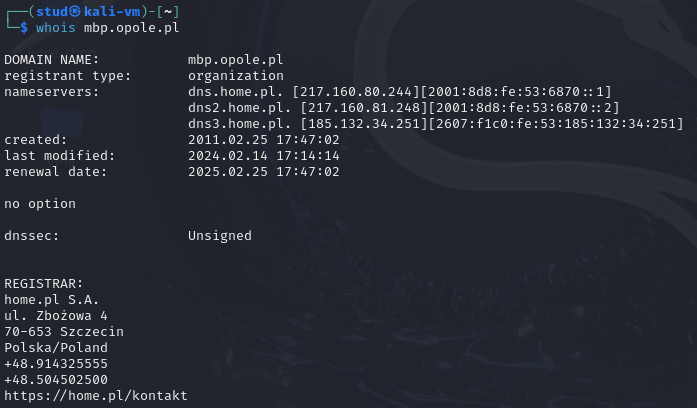
\includegraphics[width=0.6\textwidth]{whois.png}
\end{figure}

\begin{figure}[H]
  \centering
  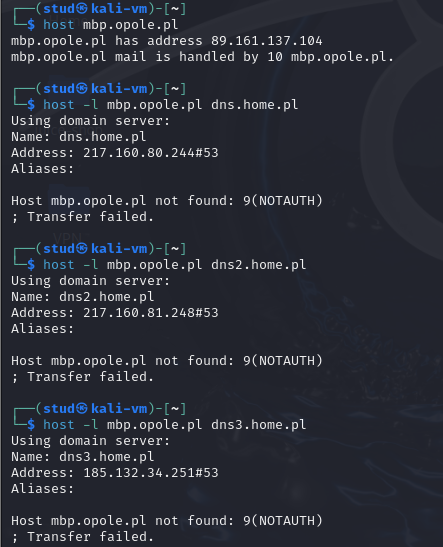
\includegraphics[width=0.6\textwidth]{host.png}
\end{figure}

\begin{figure}[H]
  \centering
  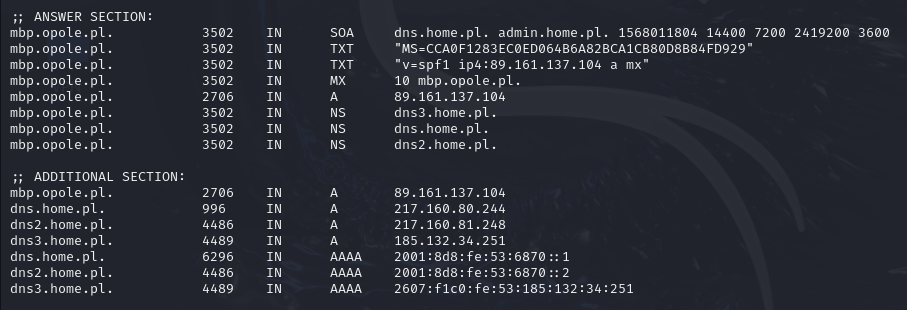
\includegraphics[width=0.6\textwidth]{dig_any.png}
\end{figure}

\begin{figure}[H]
  \centering
  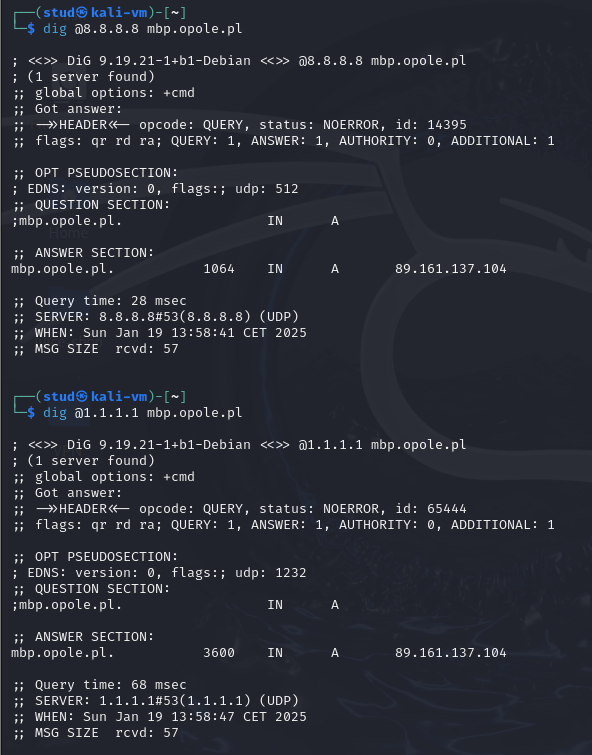
\includegraphics[width=0.6\textwidth]{dig_8888.png}
\end{figure}

\begin{figure}[H]
  \centering
  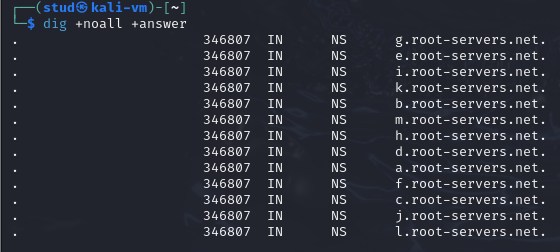
\includegraphics[width=0.6\textwidth]{dig_noall.png}
\end{figure}


\begin{itemize}
  \item Primary dns: dns.home.pl
  \item TTL: 3502s
\end{itemize}

Czas od ostatniego żądania
\begin{itemize}
  \item 8.8.8.8: ok 2500.
  \item 8.8.4.4: 347s.
  \item 1.1.1.1: 0s
  \item localhost: ok. 2400s
\end{itemize}

\begin{figure}[H]
  \centering
  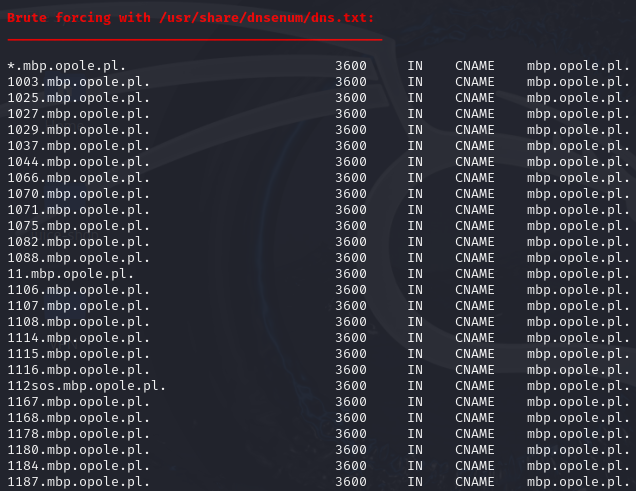
\includegraphics[width=0.6\textwidth]{dnsenum.png}
\end{figure}

\begin{figure}[H]
  \centering
  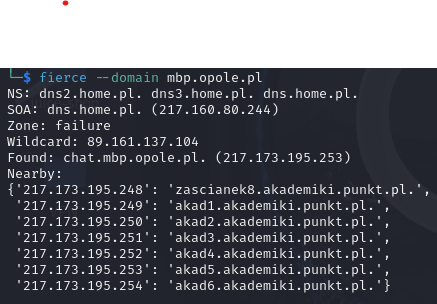
\includegraphics[width=0.6\textwidth]{fierce.png}
\end{figure}

\begin{figure}[H]
  \centering
  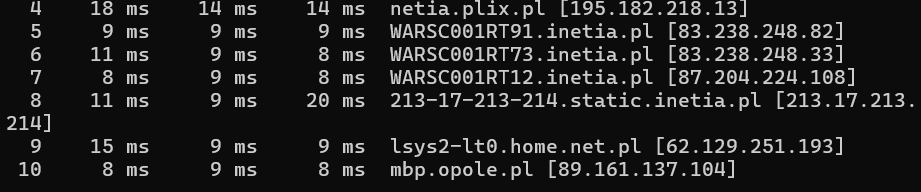
\includegraphics[width=0.6\textwidth]{traceroute.png}
\end{figure}


Za pomocą wyżej przedstawionych komend można uzyskać wiele istotnych informacji. 
Dla przykładu polecenie whois pozwala na uzyskanie informacji o założycielu domeny, dacie jej stworzenia, ostatniej modyfikacji.
Polecenie host pozwala na rozwiązanie nazwy DNS, traceroute pokazuje scieżkę pakietów w sieci i pozwala zidentyfikować węzły przez jakie przechodzi rządanie do danego hosta.
Wykorzystanie polecenia dig mx pozwala na uzyskanie informacji dotyczących serwerów pocztowych domeny. Z kolei dnsenum pozwala na uzyskanie informacji dotyczących usług, które znajdują się na serwerze.
Za pomocą komendy fierce możemy przeprowadzić testy penetracyjne, ujawniające rekordy DNS dla danej domeny i odkrycie subdomen. 

Nardzędziem, które może być najbardziej wszechstronne i przydatne wydaje się dnsenum - pozwala na kompleksową analizę DNS, dającą informacje
dotyczące usług uruchomionych na serwerze.

Nie udało się wyszukać wrażliwych plików poprzez wyszukiwanie przeglądarkowe, jedynie dość ogólne informacje na temat biblioteki.

\begin{figure}[H]
  \centering
  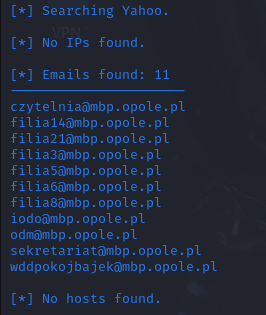
\includegraphics[width=0.6\textwidth]{harvester_yahoo.png}
\end{figure}
\begin{figure}
  \centering
  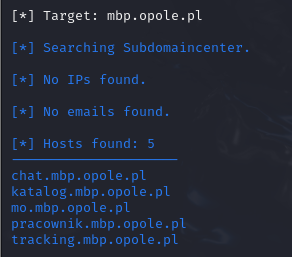
\includegraphics[width=0.6\textwidth]{harvester_subdomaincenter.png}
\end{figure}
Odnaleziono 11 adresów email związanych z yahoo, oraz 5 subdomen. Jedną z subdomen jest pracownik.mbp.opole.pl ukazujący formularz logowania.
\begin{figure}
  \centering
  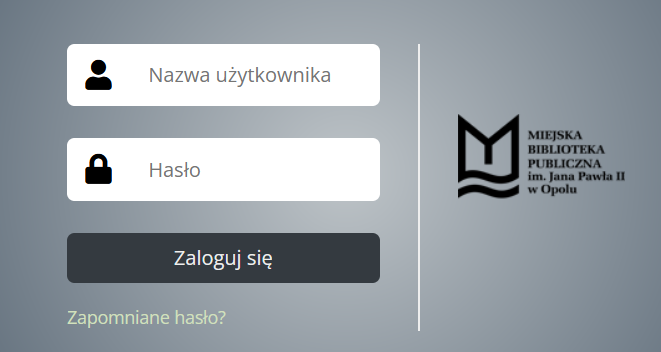
\includegraphics[width=0.6\textwidth]{pracownik_mbp.png}
\end{figure}

\section*{Krytyczne lubi w zabezpieczeniach}
\begin{itemize}
  \item CVE-2021-44228: Biblioteka Apache Log4j w wersjach 2.0-alpha1 - 2.16.0 (z wyłączeniem kilku wersji), podatność na zdalne wykonywanie kodu oraz atak odmowy dostępu. Luka była na tyle poważna, że wiele państw postanowiło wyłączyć krytyczne serwisy/strony internetowe do czasu rozwiązania problemu.
  \item CVE-2021-4045: Kamera Tp-Link Tapo C200 w wersjach oprogramowania 1.1.15 i poniżej jest podatna na wstrzykiwanie poleceń, pozwalające atakującemu na przejęcie pełnej kontroli nad kamerą. W ciągu ostatniego roku zanotowano ok. 70 ataków wykorzystujących tę lukę, najwięcej ofiar pochodzi z Japonii i Stanów Zjednoczonych.
\end{itemize}


\end{document}